% ============================================================
\section{System Design}
This chapter describes the design of the proposed system and the iterative steps that led to the final architecture. The process is presented as a sequence of design stages, where each iteration evaluates feasibility on Apple Vision Pro (AVP) and measures progress against the project requirements. Key decisions are justified by the constraints of the deployment context, the need for reliable 6D pose estimation from RGB-D data, and the requirement for stable visualization in both the image plane and AVP world space. The chapter therefore focuses not only on what was built, but also on why specific architectural choices were made.

\subsection{Early Challenges and Design Evolution}

\subsubsection{Early Challenges}
The target platform is AVP under the standard Apple Developer Program (ADP), where key sensor interfaces are gated behind extended entitlements available only through the Apple Developer Enterprise Program (ADEP). Consequently, direct access to raw RGB frames, depth sensing, camera intrinsics, and pixel-to-world mapping is unavailable. This ruled out the initial ``AVP-sensor-first'' pipeline and motivated a redesign toward screen-mirrored RGB acquisition and an external RGB-D sensor for metric depth. Table~\ref{tab:adep_blocked} summarizes the blocked features and resulting design implications.

\begin{table}[H]
    \centering
    \caption{Features only accessible through the Apple Developer Enterprise Program}
    \label{tab:adep_blocked}
    \begin{tabular}{p{0.45\linewidth}p{0.45\linewidth}}
        \toprule
        \textbf{Feature} & \textbf{Workaround} \\
        \midrule
        AVP RGB camera feed & RGB obtained via AirPlay mirroring (UxPlay). \\
        AVP depth sensing & metric depth obtained via external RealSense sensor. \\
        Camera intrinsics & estimated via calibration procedure and stored as JSON. \\
        Direct pixel-to-world mapping & requires indirect registration (ArUco + device anchor). \\
        \bottomrule
    \end{tabular}
\end{table}
\subsubsection{Design Evolution}
\label{subsec:design_evolution}

Despite these constraints, the system objectives remained unchanged: estimate accurate 6D object poses from RGB-D data, provide stable pose visualization in the image plane and in AVP world space, separate camera-frame pose accuracy from world-alignment (registration) error, and support intuitive user interaction for ROI definition and calibration. 

Figure \ref{fig:initsysdesign} illustrates the initial design, which assumed direct access to AVP camera/sensor streams. Under that concept, the visionOS client would provide RGB(-D) observations and device tracking, and the backend would mainly serve mesh models and forward FoundationPose requests.

\begin{figure}[H]
  \centering
  \includegraphics[width=\textwidth]{figures/avp.png}
  % \caption[Final system architecture]{Final system architecture: visionOS frontend (interaction, configuration, head pose streaming) and Python backend (UxPlay RGB acquisition, RealSense reprojection, mask generation, FoundationPose orchestration, and diagnostics).}
  \caption[Initial system design]{Initial system design}
  \label{fig:initsysdesign}
\end{figure}
\newpage
After access restrictions were confirmed (i.e., no ADEP entitlements), the architecture was revised to acquire RGB externally via AirPlay mirroring (UxPlay), obtain metric depth through an external depth estimation approach, and move camera-to-camera registration and depth reprojection to a Python backend.

Early AR interface drafts were produced to establish the intended interaction flow before the final visionOS implementation stabilized. The main concept was a minimal ``control hub'' that exposes only essential configuration (e.g., CAD/model selection and ROI parameterization) while delegating detailed operations to auxiliary views. Figure~\ref{fig:legacy_main_ui} shows the legacy main UI draft that motivated this separation.

\begin{figure}[H]
    \centering
    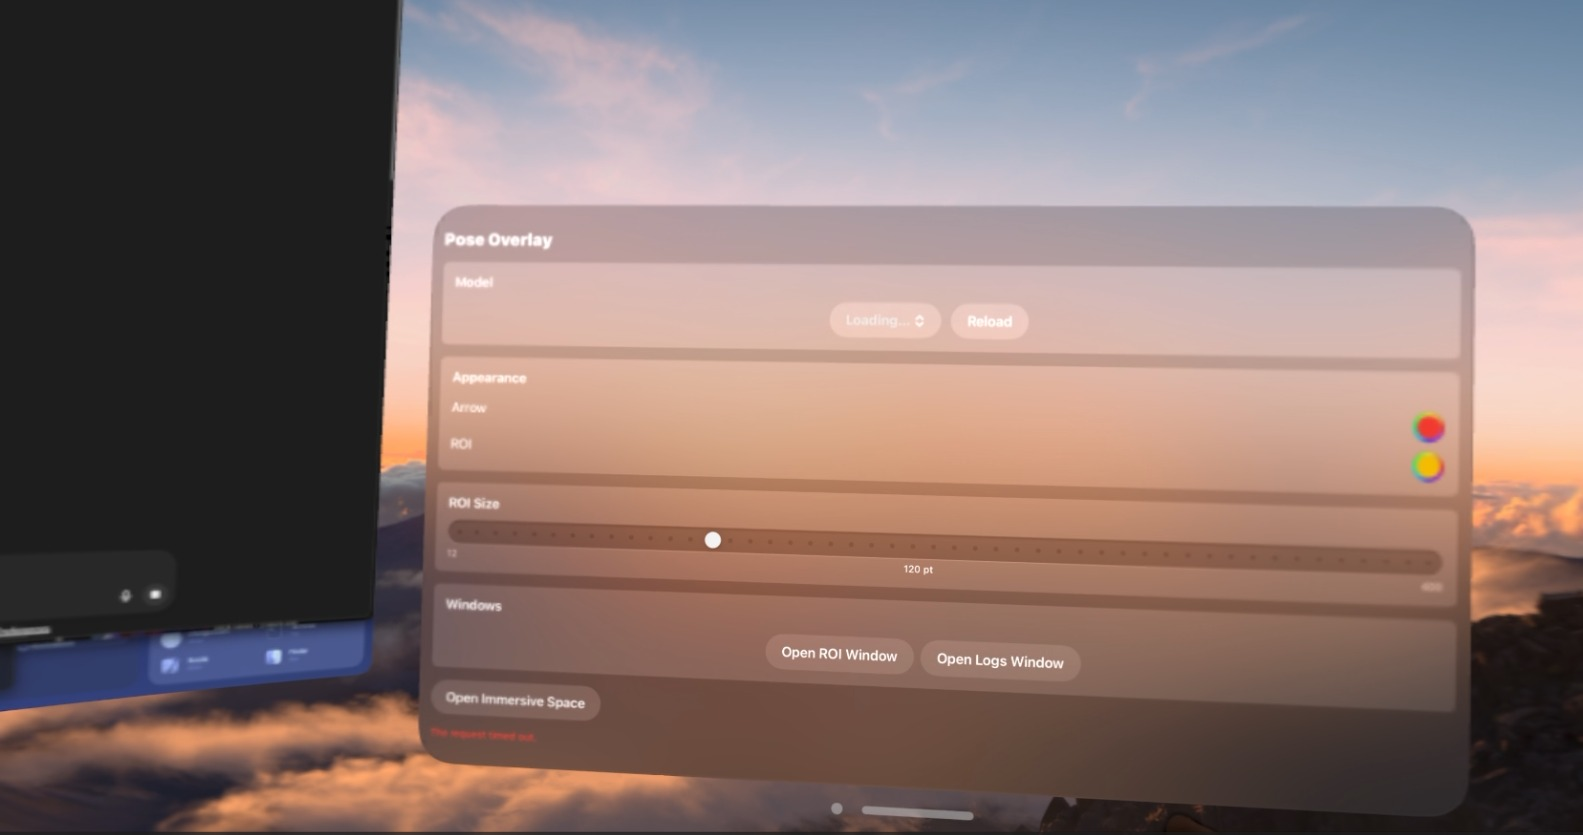
\includegraphics[width=\textwidth]{figures/legacymainui.png}
    \caption[Legacy main AR UI]{Legacy main AR UI draft}
    \label{fig:legacy_main_ui}
\end{figure}
Two legacy ROI editor concepts were explored to generate a binary mask suitable for backend requests from an RGB stream. The first concept uses a ring-shaped ROI as a lightweight approximation for isolating the target region, while the second supports freeform ROI definition for cases where circular assumptions are insufficient. Both designs served as exploratory UI artifacts and were not carried into the final system unchanged. Figure~\ref{fig:legacy_roi_editors} summarizes both concepts.

\begin{figure}[H]
    \centering
    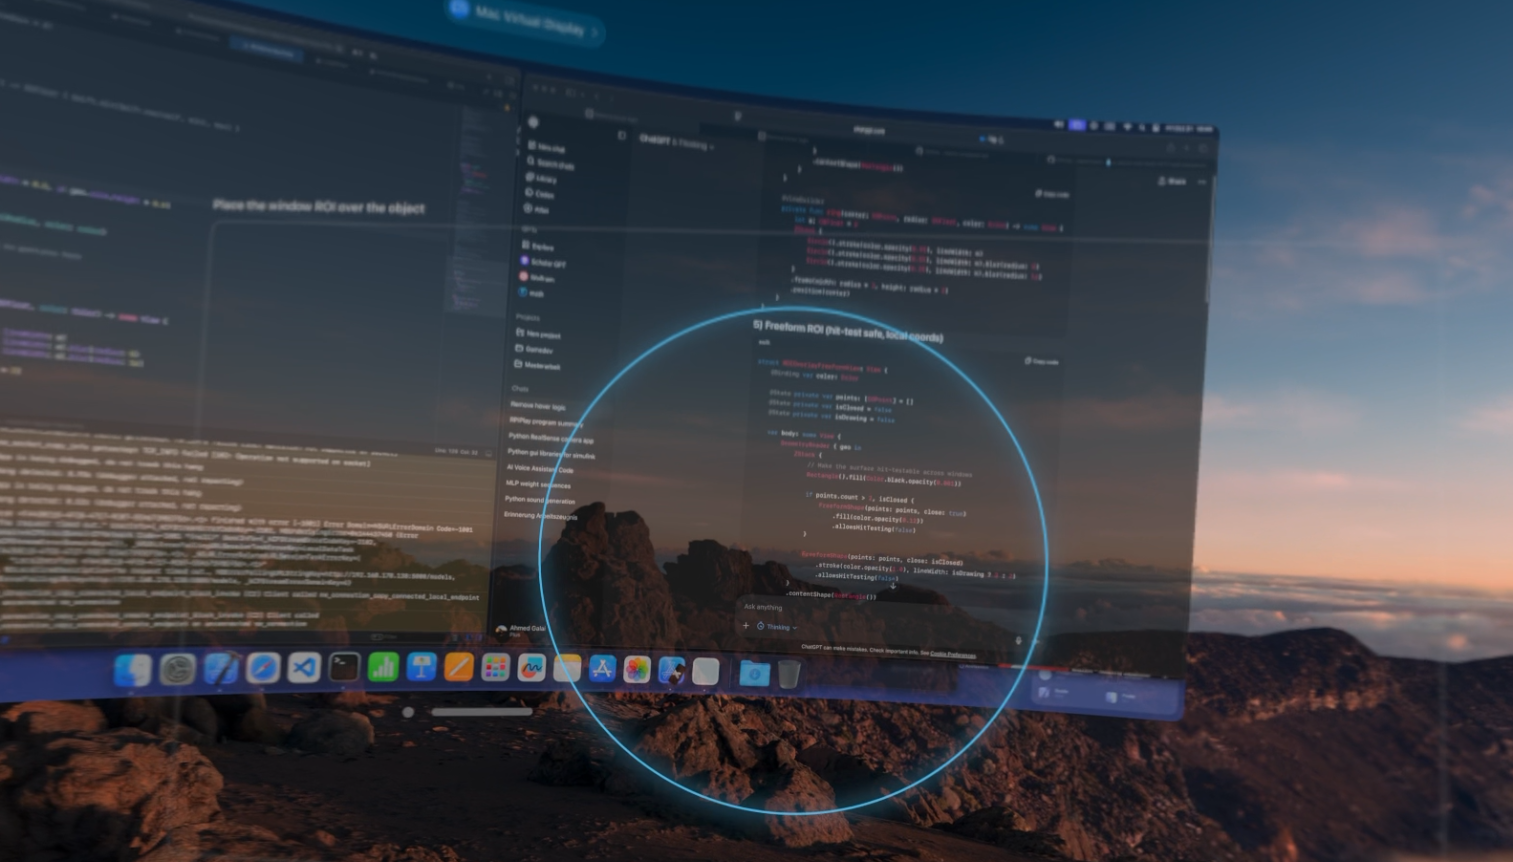
\includegraphics[width=0.49\textwidth]{figures/legacyringroi.png}
    \hfill
    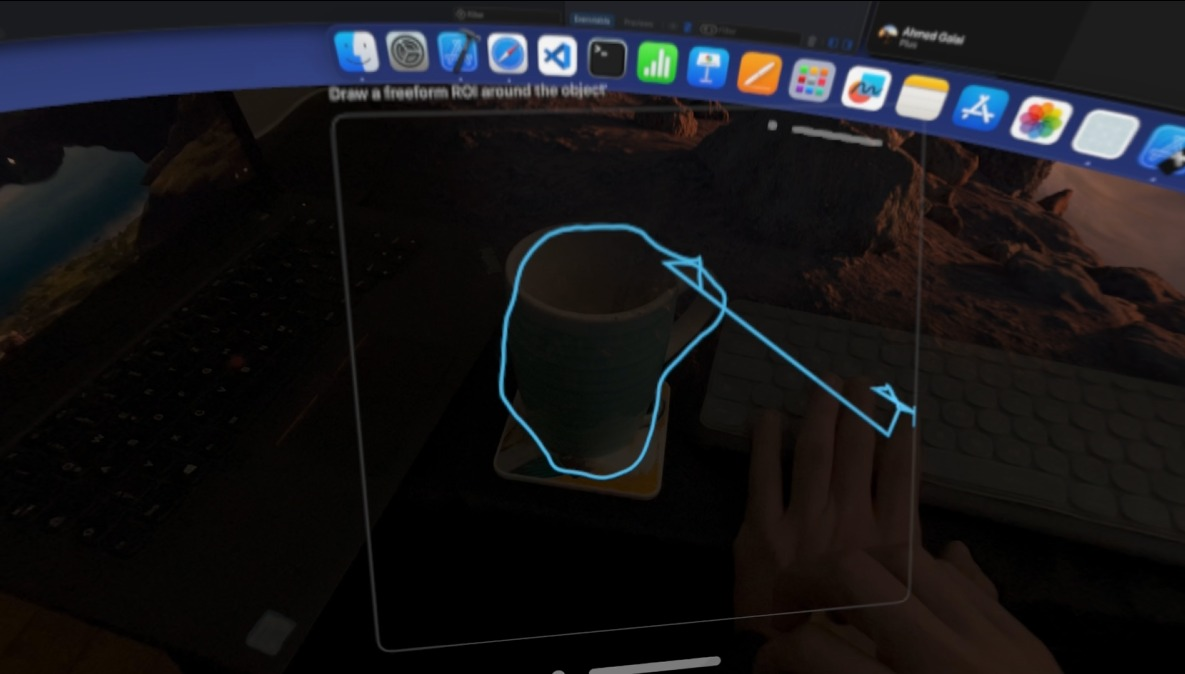
\includegraphics[width=0.49\textwidth]{figures/freeformroi.png}
    \caption[Legacy ROI editors]{Legacy ROI editor drafts: ring-shaped ROI selection (left) and freeform ROI selection (right), each providing preview and mask output.}
    \label{fig:legacy_roi_editors}
\end{figure}

To enable early end-to-end testing without relying on restricted AVP camera and sensor access under ADP, a Python-based prototype was implemented as a stand-in client for the planned perception pipeline. It enabled rapid iteration on intrinsic calibration, ROI definition, depth sourcing, payload construction, and client--server integration with either a pose estimation API or a mock interface with compatible inputs and outputs.

A central prerequisite for pose estimation and visualization is the availability of an object mesh. Before calibration, the prototype therefore allows selecting a 3D model from a backend model directory via a dropdown menu. The available assets include publicly available meshes and basic geometric primitives generated through Python scripts, with most selections aligned to objects used in the FoundationPose benchmark to remain consistent with common evaluation settings. After selection, the mesh is loaded at runtime and visualization-related quantities are precomputed, including mesh edges, center of mass, and a reference axis length. Example models are shown in Figure~\ref{fig:python_prototype_models}.

\begin{figure}[H]
    \centering
    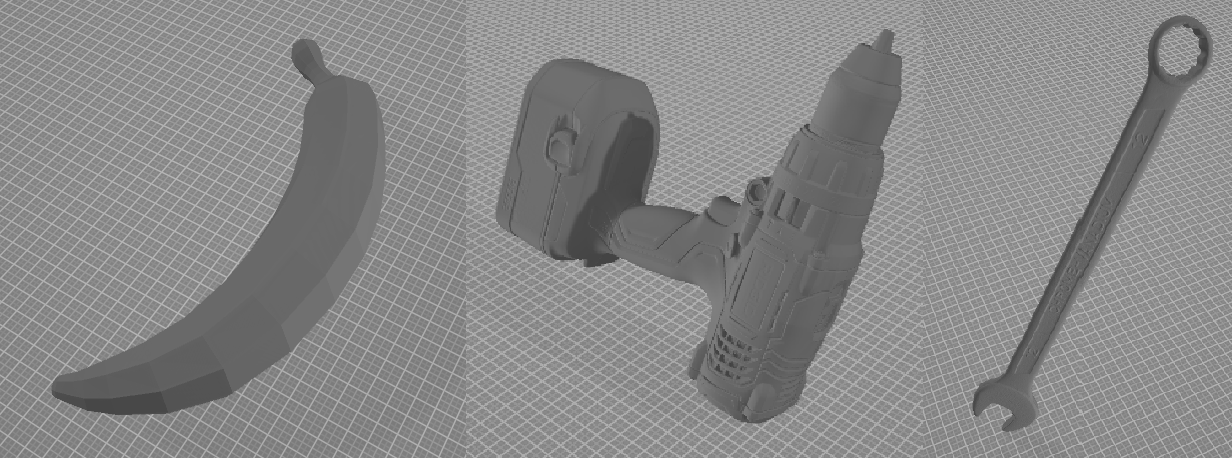
\includegraphics[width=0.9\textwidth]{figures/plymodels.png}
    \caption[Prototype 3D models]{Example 3D mesh models used in the prototype (banana, electric drill, spanner).}
    \label{fig:python_prototype_models}
\end{figure}

The calibration and ROI setup workflow is illustrated in Figure~\ref{fig:python_prototype_tab1}. This view combines the model selector with stereo image capture for intrinsic estimation and provides a rectified image canvas used to define the ROI. The rectified view serves as a practical check that the estimated intrinsics yield consistent image geometry before proceeding to depth and pose tests.

\begin{figure}[H]
\centering
\fbox{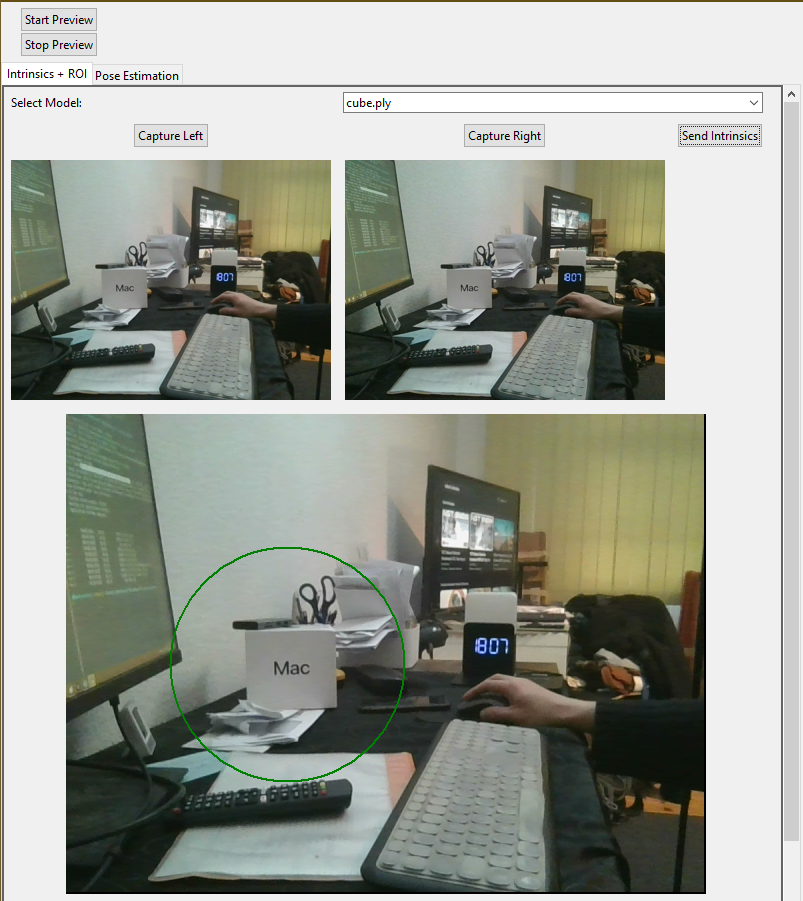
\includegraphics[width=0.8\textwidth]{figures/basiypythonclient.png}}
\caption[Python prototype: calibration]{Python prototype view for intrinsic calibration and ROI setup (model selection, stereo capture, rectified ROI canvas).}
\label{fig:python_prototype_tab1}
\end{figure}

Runtime integration is summarized in Figure~\ref{fig:python_prototype_tab2}. The interface combines a live RGB stream, a depth visualization produced by the selected depth source, a pose overlay panel rendering the mesh wireframe and axes, an ROI-masked input preview, and a log panel for request/response inspection. Together, these views were used to validate data flow correctness and to debug failure modes prior to integrating the same modules into the visionOS frontend.

\begin{figure}[H]
\centering
\fbox{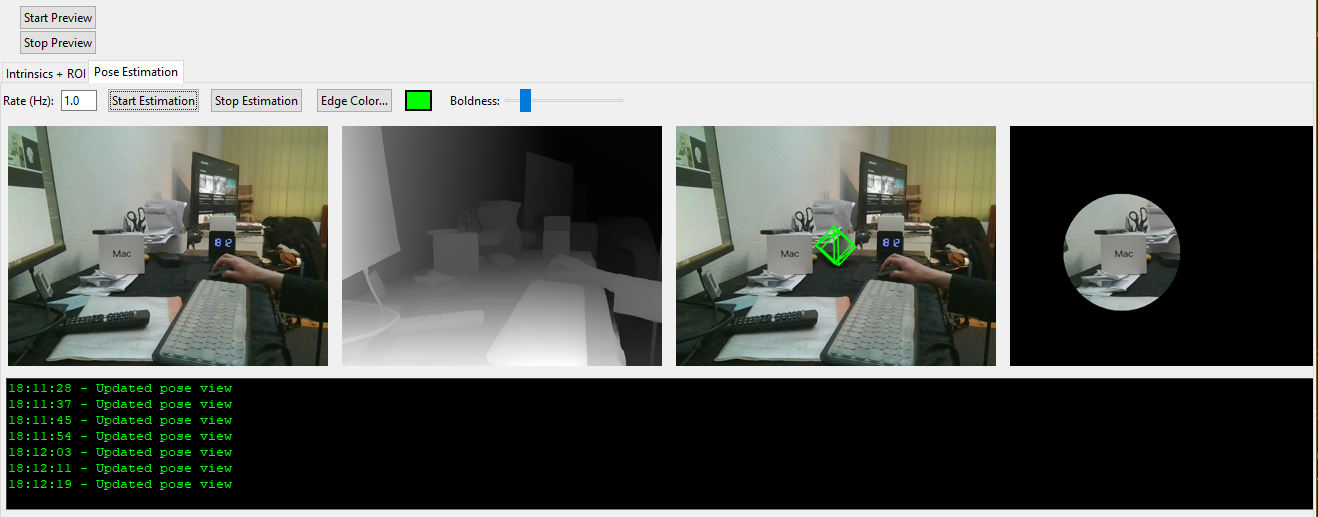
\includegraphics[width=\textwidth]{figures/basiypythonclient_2.png}}
\caption[Python prototype: runtime]{Python prototype view for runtime integration (RGB stream, depth visualization, pose overlay, ROI-masked input, API log).}
\label{fig:python_prototype_tab2}
\end{figure}

Figure~\ref{fig:depth_sources_comparison} contrasts the two depth sources considered during development: transformer-based monocular depth estimation (MDE) and metric depth from a RealSense sensor. MDE was evaluated as an intermediate solution to unblock early experiments; while the depth maps appeared visually plausible, scale ambiguity and frame-to-frame instability were observed in practice, which reduced the reliability of downstream $6$D pose estimation.

\begin{figure}[H]
\centering
\includegraphics[width=\textwidth]{figures/mde_rs_depth.png}
\caption[Depth sources comparison]{Qualitative comparison of depth sources: transformer-based monocular depth estimation (left) and RealSense metric depth after alignment (right).}
\label{fig:depth_sources_comparison}
\end{figure}

The final pipeline therefore uses a RealSense sensor to obtain metric depth. RealSense depth is first registered to the RealSense color stream using the vendor SDK. The relative pose between the RealSense camera and the mirrored AVP RGB view is then estimated from an ArUco board that is visible to both cameras, yielding a camera-to-camera transformation. Using this transform, the registered RealSense depth is reprojected into the mirrored AVP RGB frame, resolving visibility through z-buffering. A full derivation of the reprojection and the z-buffering procedure is provided in Appendix~\ref{app:math_full}.


\newpage
\subsection{Final System Architecture}
\label{subsec:final_arch}

Figure~\ref{fig:sysdesign} shows the final architecture split into a \emph{Frontend} (visionOS client) and a \emph{Backend} (Python services). This figure replaces earlier ``AVP-sensor-first'' concepts.

\begin{figure}[H]
  \centering
  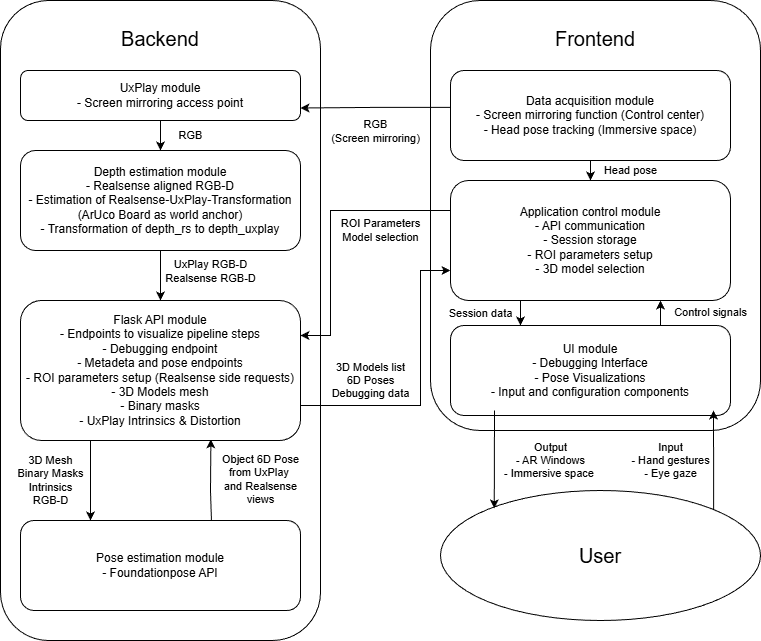
\includegraphics[width=\textwidth]{figures/System_diagram.png}
  \caption[Final system architecture]{Final system architecture: visionOS frontend (interaction, configuration, head pose streaming) and Python backend (UxPlay RGB acquisition, RealSense reprojection, mask generation, FoundationPose orchestration, and diagnostics).}
  % \caption[Final system architecture]{Final system architecture}
  \label{fig:sysdesign}
\end{figure}

The system is split into a lightweight visionOS frontend and a Python backend to match platform constraints and to separate interaction from pixel-level computation. The visionOS client is intentionally thin in terms of perception and acts as the user-facing control layer: it manages session state, hand-gesture and eye-gaze interaction for region-of-interest (ROI) definition, object/model selection, and runtime configuration. It also streams the head/device pose to the backend to support world registration and stable overlays as the user moves. Pose outputs returned by the backend are visualized either as optional 2D annotations in the image plane or as 3D augmentations in immersive space.

The backend performs all pixel-domain processing and inference orchestration. It receives the mirrored AVP RGB stream via UxPlay and buffers frames, while also acquiring RealSense RGB-D and aligning depth to the RealSense color stream using the vendor SDK. The camera-to-camera transform $\mathbf{T}_{AVP \leftarrow RS}$ is estimated from paired ArUco detections and used to reproject aligned RealSense depth into the mirrored AVP view with z-buffering. Given normalized ROI parameters from the client, the backend generates binary masks in AVP image coordinates, assembles payloads for FoundationPose, and returns $6$D pose estimates to the frontend. Diagnostic endpoints (e.g., intermediate visualizations and a debug dashboard) are provided to inspect registration, masks, reprojected depth, and pose overlays during testing.

\subsubsection{ROI Design and Mask Generation}
\label{subsec:design_roi}
ROI definition and mask generation underwent several iterations, primarily driven by robustness issues observed during integration with the mirrored RGB stream.

Early iterations relied on a movable AR overlay window that rendered either a colored ring or a freeform contour on top of the mirrored RGB view. The backend reconstructed a binary mask by applying HSV thresholding to isolate the overlay color in the mirrored frame and then converting the detected outline into a filled region. Illustrations of these concepts are provided in earier this chapter (Figure~\ref{fig:legacy_roi_editors}). In practice, this approach proved brittle: HSV thresholds required frequent adjustment due to changes in illumination and mirroring artifacts, and small errors in outline extraction produced invalid or noisy masks. Replacing the outline with a filled disc improved stability, but occluded relevant object pixels in the mirrored image and reduced pose estimation accuracy.

The final system represents the ROI as normalized parameters $(c_x, c_y, r)$ transmitted directly to the backend. The ROI window is retained only as an alignment aid; mask generation is performed analytically on the backend, eliminating dependence on HSV reconstruction and outline extraction. Figure~\ref{fig:roi_final_window_placeholder} shows the final ROI setup window.

\begin{figure}[H]
    \centering
    \includegraphics[width=\textwidth]{figures/roi_windw_final.png}
    \caption[Final ROI setup window]{Final ROI setup window used to align the normalized circular ROI before pose capture.}
    \label{fig:roi_final_window_placeholder}
\end{figure}

A side effect of rendering the ROI window over mirrored content is an ``infinite mirror'' artifact when the overlay is captured inside the mirrored stream. In practice, the ROI is adjusted while the overlay is visible and the ROI window is closed before pose capture, avoiding recursive artifacts in the backend input.

\subsubsection{Pipeline Stages and Overlay Strategy}
\label{subsec:design_pipeline_and_overlay}

The original target was to render pose overlays directly in AVP world space. Under ADP constraints, the design prioritizes 2D visualization in the mirrored RGB view as the primary debugging and validation mode, since camera-frame consistency can be verified directly in the image plane and the result is largely decoupled from world-registration drift. Once camera-frame behavior is stable, the same pose estimates can be rendered as immersive 3D overlays, which requires calibration of the device-to-camera relationship and reliable marker-based registration Table~\ref{tab:cv_stages_final} summarizes the effective pipeline stages in the final design.

\begin{table}[H]
    \centering
    \caption[Final pipeline stages]{Pipeline stages in the final system.}
    \label{tab:cv_stages_final}
    \begin{tabular}{p{0.24\linewidth}p{0.62\linewidth}}
        \toprule
        \textbf{Stage} & \textbf{Description} \\
        \midrule
        UxPlay RGB acquisition &
        Mirrored AVP frames are received and buffered by the backend. \\
        RealSense RGB-D acquisition &
        RealSense streams are captured; depth is aligned to color via SDK. \\
        Camera-to-camera registration &
        Paired ArUco detections yield $\mathbf{T}_{AVP \leftarrow RS}$. \\
        Depth reprojection &
        Aligned depth is transformed into the UxPlay view (z-buffering). \\
        ROI mask synthesis &
        Backend generates binary masks from normalized $(c_x,c_y,r)$. \\
        Pose inference &
        FoundationPose outputs $\mathbf{T}_{C \leftarrow O}$ per frame. \\
        Visualization &
        2D overlays in UxPlay view and/or 3D overlays in immersive space. \\
        \bottomrule
    \end{tabular}
\end{table}
\newpage
The most relevant transforms used by these stages are summarized here for reference. Homogeneous transforms are written as
\[
\mathbf{T}_{A \leftarrow B} =
\begin{bmatrix}
\mathbf{R}_{AB} & \mathbf{t}_{AB} \\
\mathbf{0}^\top & 1
\end{bmatrix},
\qquad
\mathbf{X}_A = \mathbf{R}_{AB}\mathbf{X}_B + \mathbf{t}_{AB}.
\]
Camera intrinsics follow the pinhole model
\[
\mathbf{K} =
\begin{bmatrix}
f_x & 0 & c_x \\
0 & f_y & c_y \\
0 & 0 & 1
\end{bmatrix}.
\]
ArUco detections provide $\mathbf{T}_{C \leftarrow M}$ for each camera, and the RealSense-to-AVP transform used for depth reprojection is computed as
\[
\mathbf{T}_{AVP \leftarrow RS} =
\mathbf{T}_{AVP \leftarrow M}\left(\mathbf{T}_{RS \leftarrow M}\right)^{-1}.
\]
Aligned RealSense depth is back-projected into 3D and transformed into the AVP/UxPlay frame via
\[
\mathbf{X}_{RS} = z\,\mathbf{K}_{RS}^{-1}
\begin{bmatrix}
u \\ v \\ 1
\end{bmatrix},
\qquad
\mathbf{X}_{AVP} = \mathbf{R}_{AVPRS}\mathbf{X}_{RS} + \mathbf{t}_{AVPRS},
\]
followed by projection into the UxPlay image plane using $\mathbf{K}_{AVP}$, with visibility resolved through z-buffering:
\[
depth_{UxPlay}(v,u) = \min\{ z_{AVP} \mid (u_{AVP},v_{AVP})=(u,v),\ z_{AVP}>0 \}.
\]
For immersive 3D overlays, the device anchor provides $\mathbf{T}_{W \leftarrow D}$ and a calibrated offset $\mathbf{T}_{D \leftarrow C}$ yields
\[
\mathbf{T}_{W \leftarrow C} = \mathbf{T}_{W \leftarrow D}\mathbf{T}_{D \leftarrow C},
\]
enabling world-anchored marker and object placement as described in Appendix~\ref{app:math_full}.
